\documentclass[UTF8]{ctexart}
\usepackage{graphicx}   

\begin{document}
    36,false,因为使用SRSW规则寄存器替换会使得,被读入寄存器读出的对角线上的值或被其他读入调用时写入的对应行的值,会成为旧值,此时无法成为MRSW原子寄存器。
    
    42,代码如图,在同一时刻read,只能修改3组数中的一组,修改第一组时,第二三组一样,会读出旧值;修改第二组时,一三组不同需要循环;修改第三组是,一二组一样是新值,之后的read都会都读出新值。因此有作用。
    
    \centering
    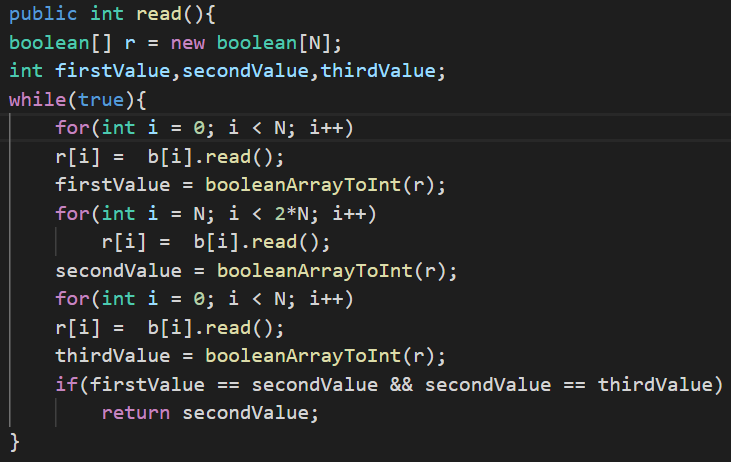
\includegraphics{./1.PNG}

\end{document}